This chapter describes a novel user interface paradigm for authoring mid-air gestures based on \emph{space discretization}, and its implementation as part of an end-to-end software tool designed to support end-users: \emph{Hotspotizer}. The design of the space discretization paradigm and Hotspotizer's user interface has been informed by insights from previously published research and the analysis of related artifacts (described in Chapter~\ref{chp:background}), along with the use of methods from user-centered design (described in Chapter~\ref{chp:design}).

\section{Space Discretization}

This section introduces a user interface paradigm based on space discretization for visualizing and manipulating gesture information. The essence of the paradigm is the partitioning of the interaction space into discrete cells. These discrete cells within the workspace may be marked to become hotspots – or \emph{hotspotized} – that register when a limb or input device passes through them. Multiple cells can be hotspotized to form large regions with relaxed spatial constraints; and temporal ordering between different regions can be specified to express movement. In essence, hotspots behave like virtual, invisible buttons positioned in the interaction space (Figure~\ref{fig:wave-low}).

\begin{SCfigure}[5][b]
\centering
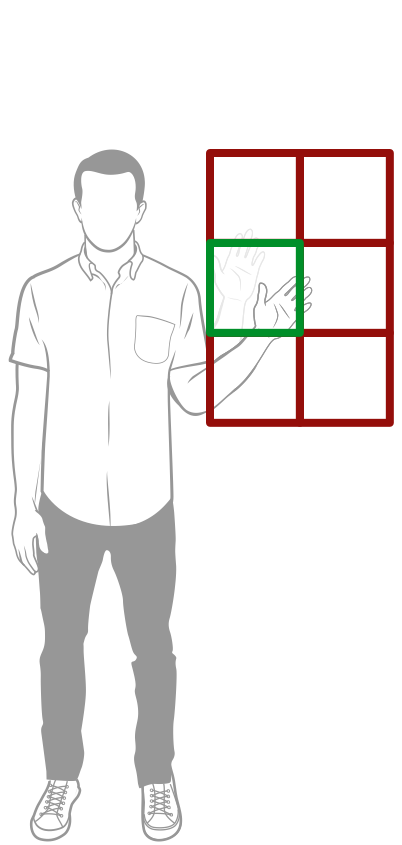
\includegraphics[width=.2\textwidth]{wave-low}
\caption{Hotspots behave like virtual buttons set in the interaction space. A wide variety of gestures can be described in as sequences of hotspot configurations.}
\label{fig:wave-low}
\end{SCfigure}

Figure~\ref{fig:z-hotspots} shows how this paradigm can be applied to describe a gesture trajectory that follows the form of the letter \emph{Z} on a 2-dimensional surface. Four regions consisting of multiple hotspots have been defined and they must be traversed in a certain order --- indicated by the numbers on the figure --- for the gesture to register.

\begin{SCfigure}[3][t]
\centering
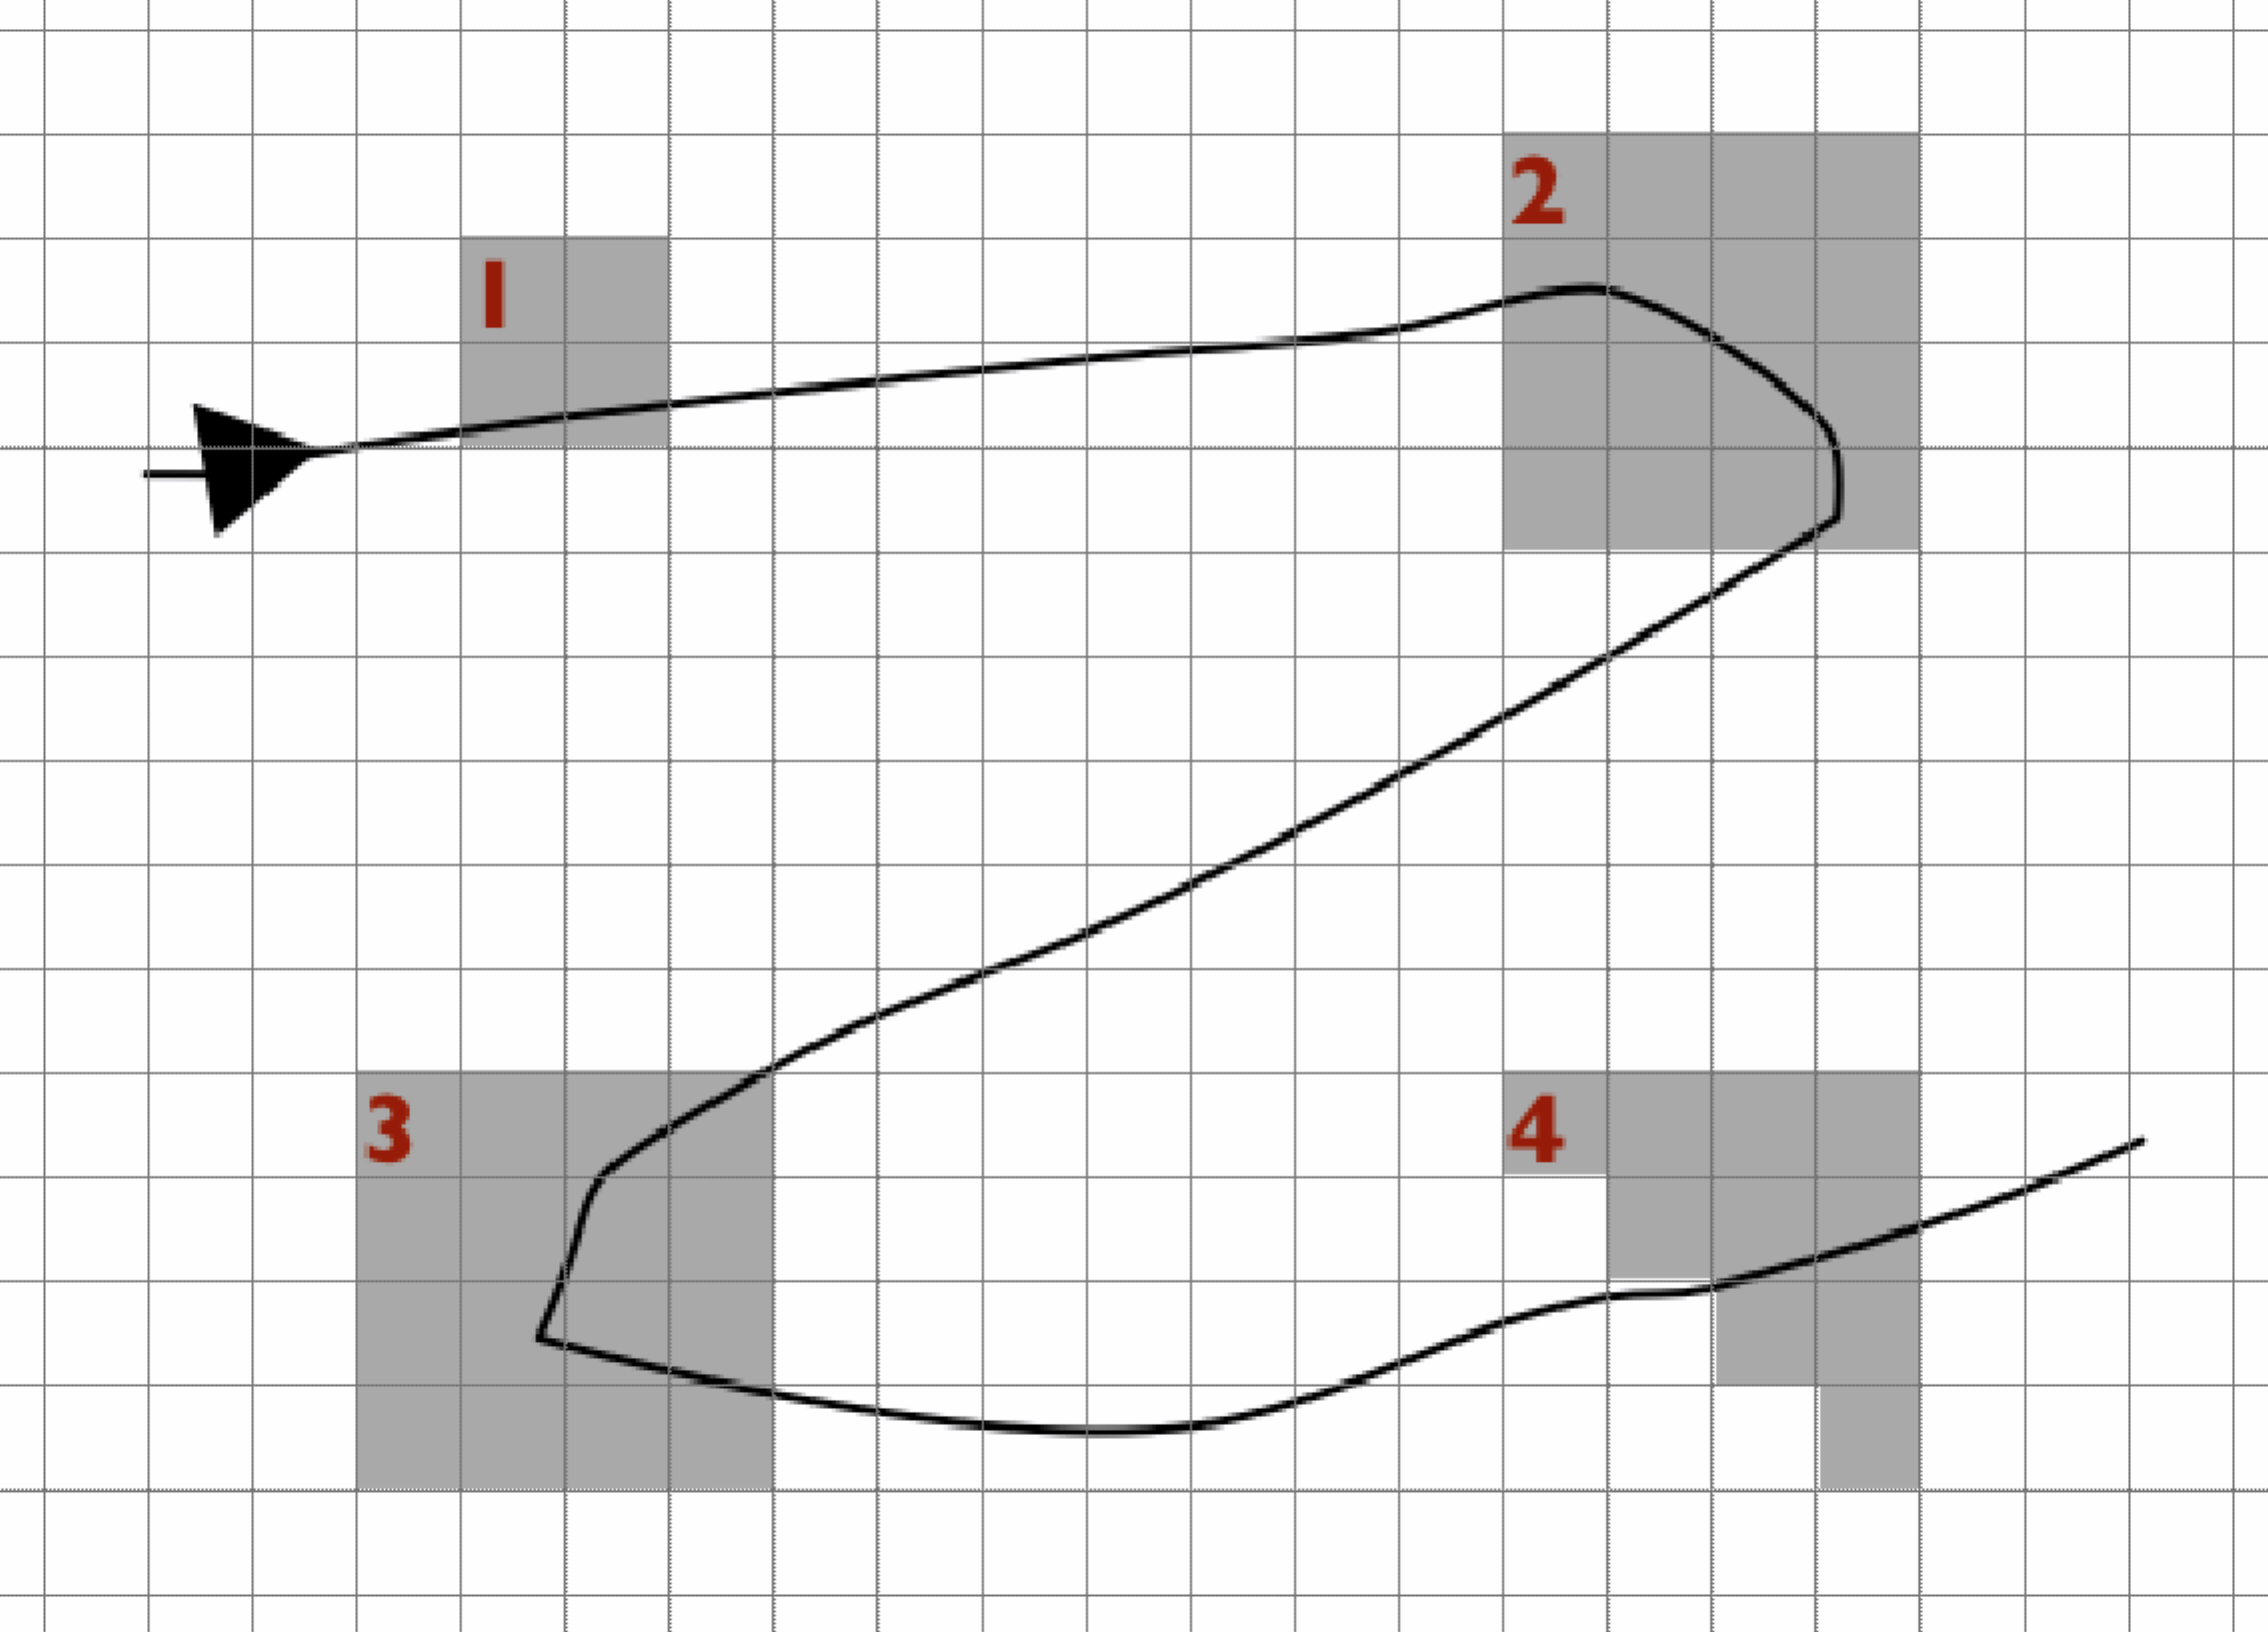
\includegraphics[width=0.4\textwidth]{z-hotspots}
\caption{A 2-dimensional surface "Z" gesture defined using ordered hotspots in discretized space.}
\label{fig:z-hotspots}
\end{SCfigure}

The paradigm is versatile in that it can be used to author gestures for a variety of capture media (see Section~\ref{sec:gestural-interaction}) ranging from touch-sensitive surfaces to perceptual interaction spaces.

The partitioned workspace must be placed in relation to a certain frame of reference. The origin of this frame of reference may be, depending on the capture medium, a certain point on a touch-sensitive surface; a camera that consists a perceptual input device; a certain limb of the user; the initial point where a stylus makes contact with a touchscreen; etc. Barring some rare cases, hotspot configurations that make up a certain gesture will differ if the origin of the workspace changes.

In line with \posscite{Shoemaker:2010} recommendation that users' sense of proprioception be leveraged within body-centric perceptual interactions (see Section~\ref{sec:design-and-evaluation-of-tools}), the hotspot array's frame of reference can originate from the user's center of gravity for applications that use coarse movements. This way, the user's position in relation to the perceptual sensor does not affect gesture recognition, as long as the sensor can build the correct skeletal model.

\begin{SCfigure}[3][b]
\centering
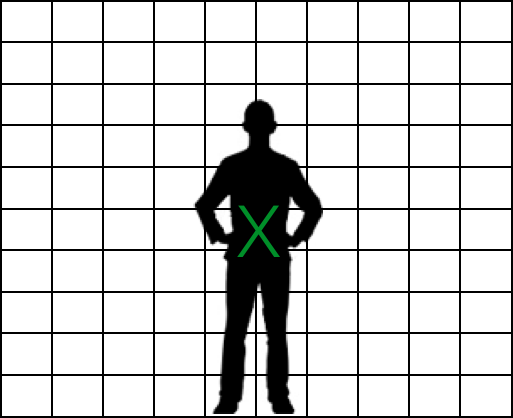
\includegraphics[width=.35\textwidth]{perceptual-grid}
\caption{For full-body perceptual interactions, the origin for the hotspot array's frame of reference can be affixed to the centroid of the user. This design leverages proprioception (see Section~\ref{sec:design-and-evaluation-of-tools}).}
\label{fig:perceptual-grid}
\end{SCfigure}

Authoring dynamic movements relies on temporal constraints between hotspots. This can take the form of a simple inter-keyframe timeout; where the time that elapses between the traversal of subsequent hotspots must not exceed a given value. A variety of visualization styles can be explored for the authoring of the temporal constraints. Using an integrated visualization that shows spatial and temporal constraints together (as in Figure~\ref{fig:z-hotspots}) is one option; as is splitting motion into discrete keyframes. With a focus on the latter option, design considerations for interacting with temporal constrains are discussed in  Sections~\ref{sec:user-interface-design} and~\ref{sec:hotspotizer}.

Gestures designed using space discretization are dependent on location, scale and orientation with respect to the workspace. Affixing the workspace to a physical part of the interactive system --- including the user's limbs --- can be exploited to introduce location and orientation invariance. For supporting scale invariance, the paradigm affords a degree of spatial flexibility; hotspotizing a larger volume of cells allows for relaxed gesture boundaries. (User studies described in Section~\ref{sec:summative-studies} have shown that using large hotspots in lieu of spatially overconstrained gesture designs is indeed a desirable --- although not inherently discoverable --- strategy.)

In essence, aspects of this technique are based on \posscite{Hoste:2013} control points paradigm, modified to confine the locations of the control points to discrete pre-defined locations and standardize the shapes of control point boundaries. Multiple areas or volumes within the workspace can be hotspotized and added together to create custom shapes. Dynamic movements can be defined by splitting motion into keyframes related by temporal or merely ordinal constraints.

\subsection{Gesture Spotting in Discretized Space}

\begin{SCfigure}[3][t]
\centering
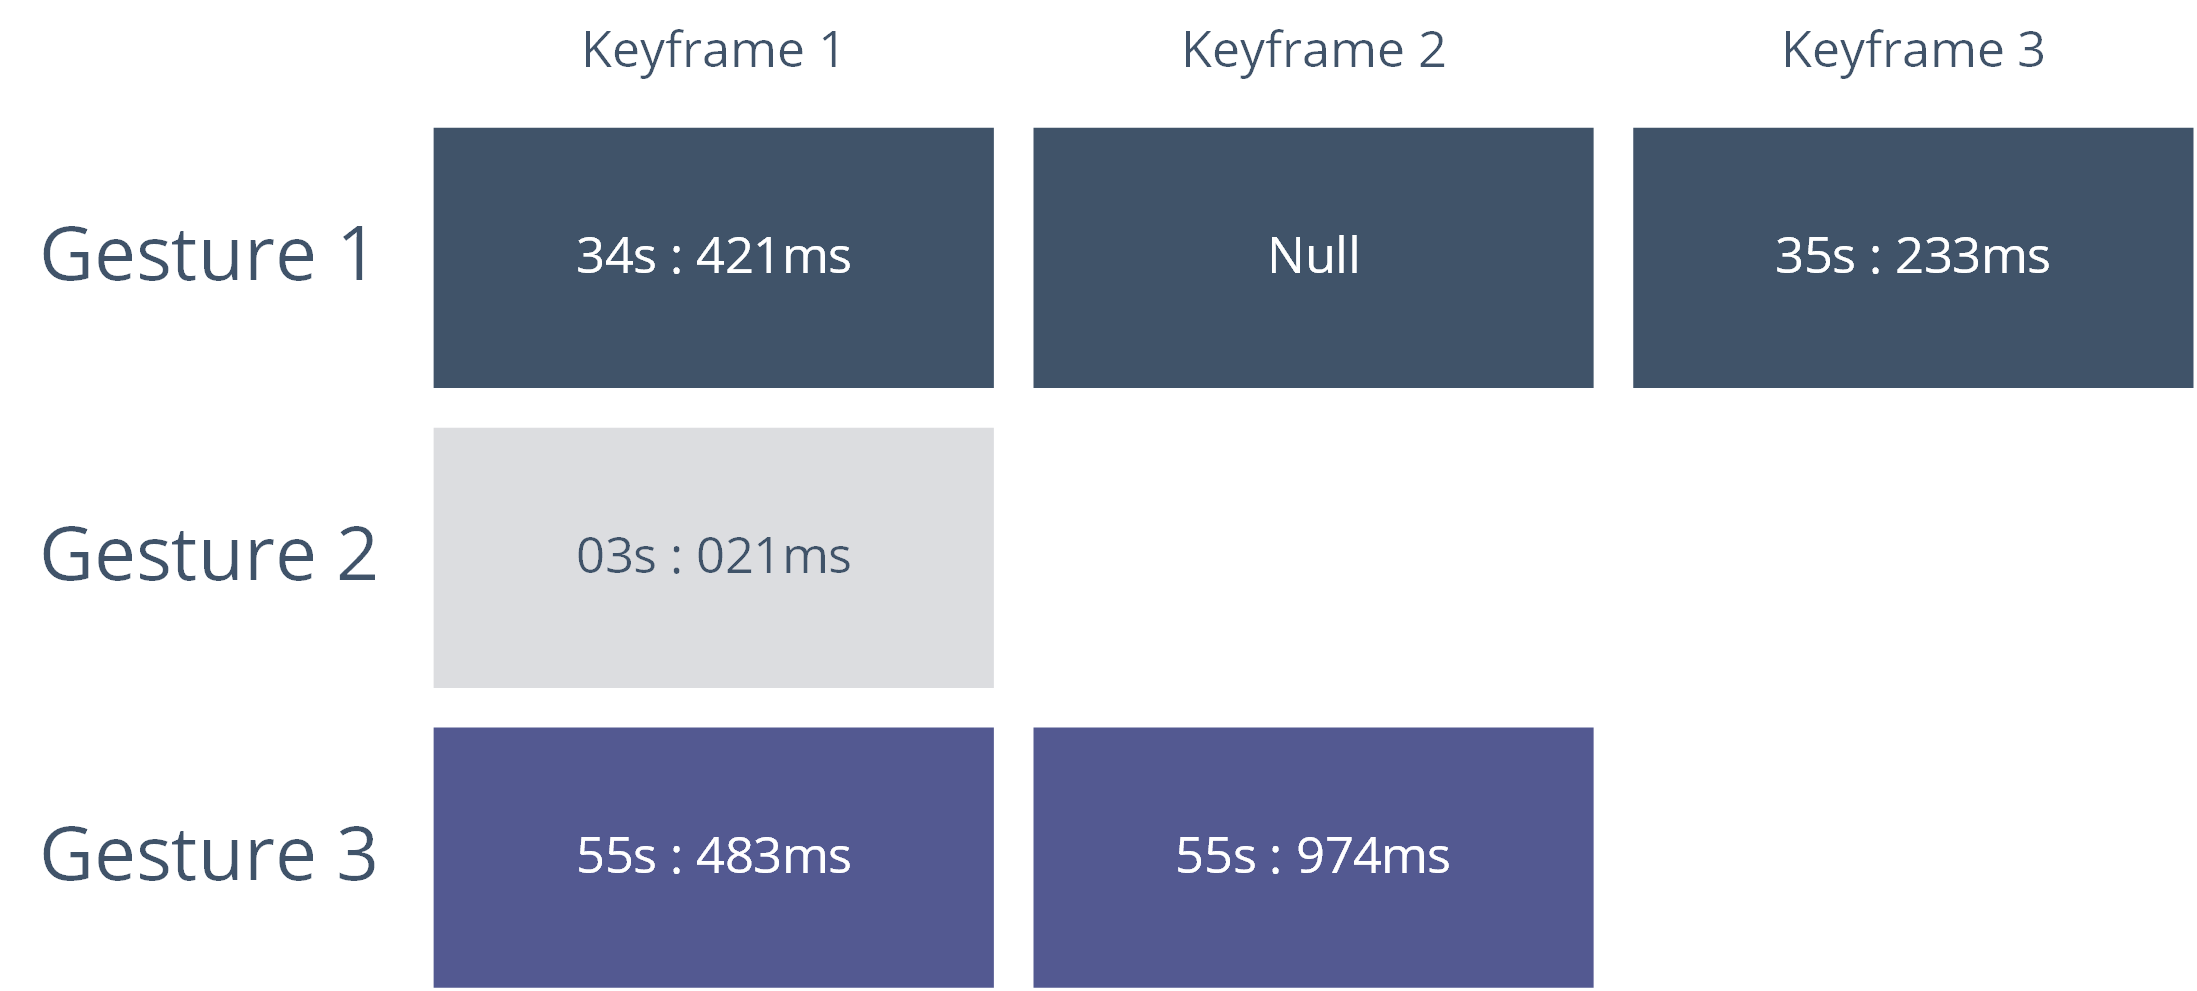
\includegraphics[width=.6\textwidth]{jagged-array}
\caption{A jagged array used to keep a memory of how tracked limbs traverse hotspots. The elements of the outer array are arrays that correspond to the gestures that the system can recognize. The elements of the inner arrays keep track of when the tracked limb last occupied the hotspots that belong to each keyframe of gesture.}
\label{fig:jagged-array}
\end{SCfigure}

The nature of perceptual user interfaces is such that input signals are often in the form of continuous streams. The continuous stream often comprises meaningful information intermingled with portions of the signal that are irrelevant or even confounding --- i.e. noise. Locating where meaningful information begins and ends within the continuous stream --- i.e. distinguishing signal from noise --- and interpreting the input signal is called \emph{spotting} \parencite{Rose:1992}. \emph{Gesture spotting} is the identification of meaningful gestures in a real-time continuous stream where gestures are performed alongside intermediate, unintentional movements \parencite{Malgireddy:2010, Kang:2004, Lee:1999, Alon:2009, Elmezain:2010}. \emph{Identification} in this sense denotes both the segmentation of meaningful portions of the stream from noise; and identifying what those meaningful portions actually mean --- i.e. \emph{classification} or \emph{labeling} in machine learning terms \parencite{Malgireddy:2010, Alon:2009}.

\begin{figure}[b]
\centering
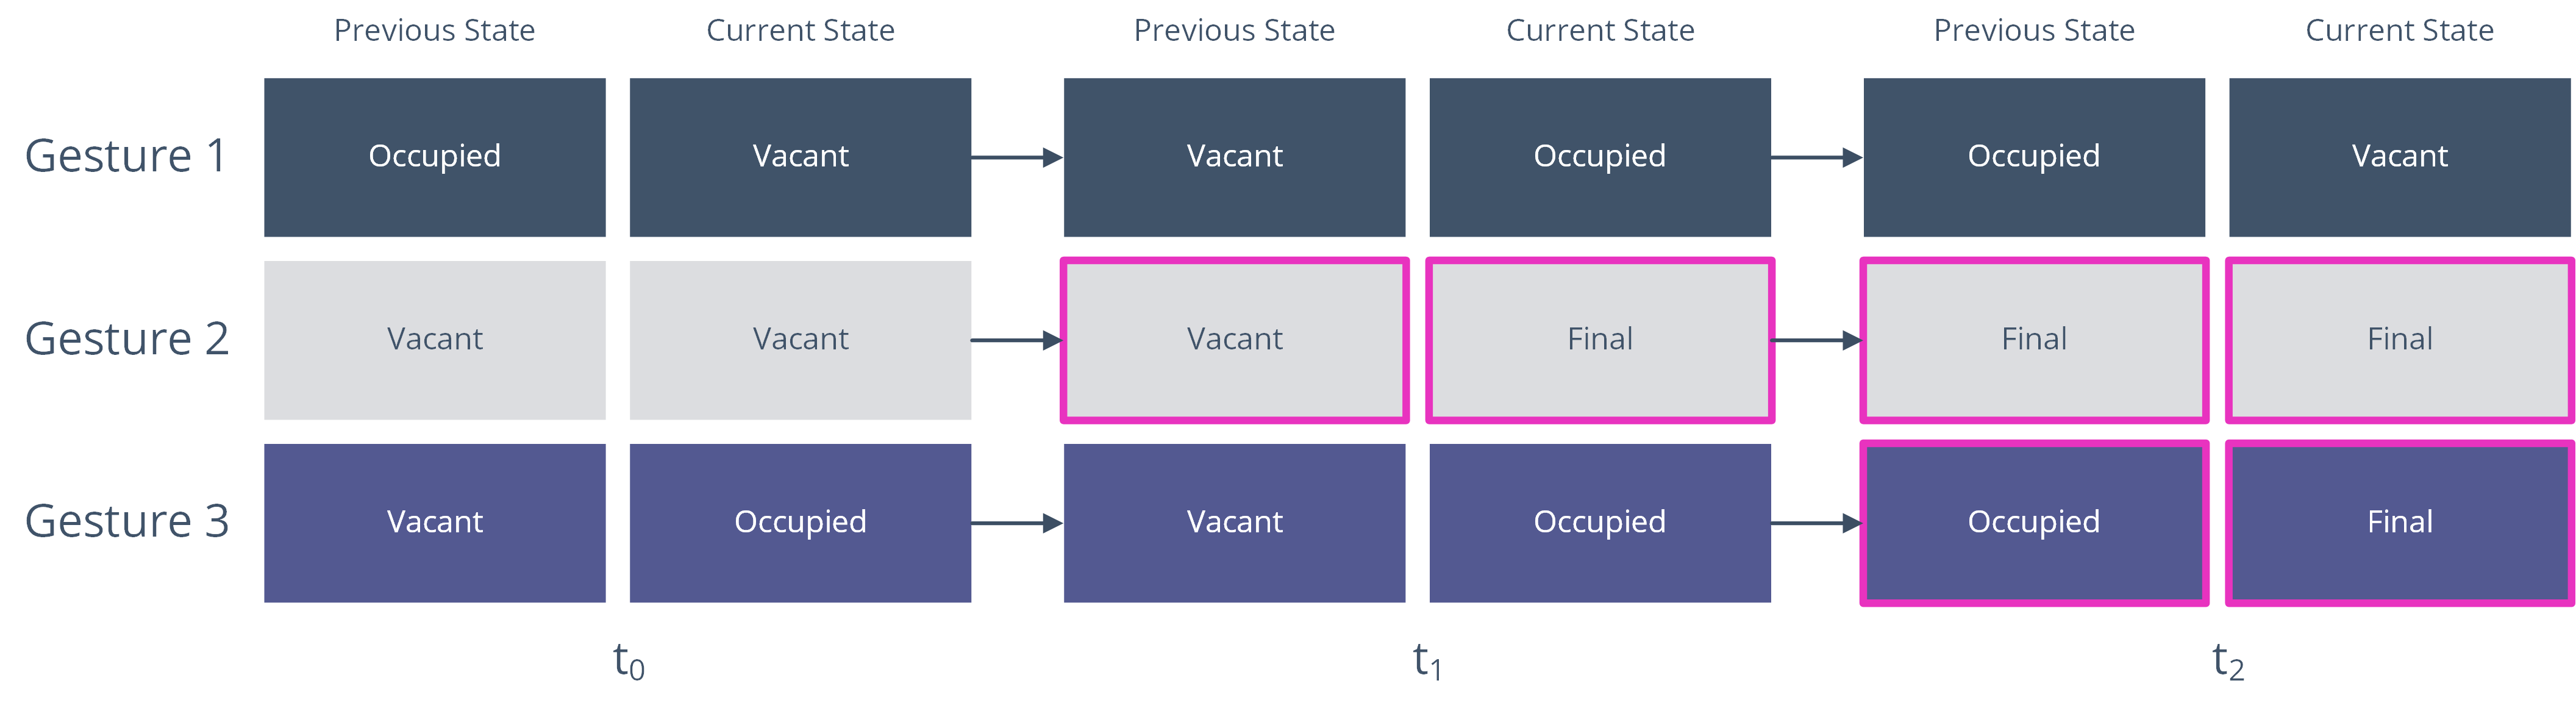
\includegraphics[width=\textwidth]{states-array}
\caption{A 2-dimensional array keeps track of what state each gesture is in. With each incoming frame from the input device, the present state expires and gets pushed back in the array to represent history. The highlights indicate candidacy for gesture recognition (Gesture 2, as in Figure~\ref{fig:jagged-array}, has one keyframe).}
\label{fig:states-array}
\end{figure}

For gesture-based interfaces, the difficulty of gesture spotting depends on the choice of capture medium (see Section~\ref{sec:gestural-interaction}). On constrained capture media, gesture segmentation is often inherent because input devices or limbs do not make contact with the gesture-sensing medium during intermediate movements. On equipped capture media, segmentation can be triggered manually, e.g. via a button on the input device. With perceptual interfaces, gesture spotting must be performed automatically. (Indeed, as \textcite{Turk:2000} imply, this one of the characteristics that define perceptual interaction.)

Defining gestures as sequences of hotspot sets in discretized space significantly alleviates the difficulties associated with perceptual gesture spotting. The interaction space consists of a finite volume, and hotspots are defined over a finite number of discrete compartments that span portions of the interaction space. Hotspots behave like virtual buttons that have two states: an \emph{on} state for when the tracked limb or input device occupies the hotspot, and an \emph{off} state for when the hotspot does not register occupation. These characteristics of operating in discretized space reduce the gesture spotting problem to one that can be solved by simple thresholding \parencite{Hoste:2013, Hartmann:2007} --- without requiring the application of machine learning concepts.

An algorithm for traversing hotspots within a workspace and performing gestures spotting can be expressed in two parts. This algorithm assumes that the interface between the input device and the application logic is event-driven, but it can adapt to a polling model as well\footnote{See  \href{http://100experiencepoints.com/polling-vs-event-driven-models/}{100experiencepoints.com/polling-vs-event-driven-models/} for a discussion on event-driven and polling interfaces between application components.}. When using the Microsoft Kinect sensor as the input device, this means that the positions of the tracked limbs that comprise the skeletal model are published to the application at regular intervals (by default, at 30 frames per second). The two parts of the algorithm are executed consecutively upon the arrival of each data frame.

\begin{lstlisting}[float=t, label=lst:part-one, caption=Part 1 of pseudocode for gesture spotting in discretized space. This part of the algorithm records the traversal of hotspots.]
# Traverse all gestures
foreach gesture in AllGestures:
  i = AllGestures.IndexOf(gesture)
  # Advance gesture state
  States[i][0] = States[i][1]
  # Traverse each keyframe of the current gesture
  foreach keyframe in gesture.Keyframes:
    j = gesture.Keyframes.IndexOf(keyframe)
    # See if the limb tracked by the current gesture
    # occupies the any hotspotized areas for this keyframe
    if keyframe.Bounds.Contain(gesture.TrackedLimb.Coordinates):
      # If it does, record *when*
      Times[i][j] = TimeOfNow
      # Also check if this is the last keyframe
      # and set gesture state
      if keyframe == gesture.Keyframes.Last:
        States[i][1] = Final
      else:
        States[i][1] = Occupied
    # If this keyframe does not register any activity...
    else:
      # Set the gesture state accordingly
      States[i][1] = Vacant
\end{lstlisting}

A second assumption of the algorithm is that temporal constraints that separate keyframes are defined in terms of a fixed inter-keyframe timeout value. For a gesture to register, hotspots that belong to its consecutive keyframes must be traversed before the timeout occurs.

The first part of the algorithm is a loop that traverses hotspots and checks if the hotspot is occupied by a limb that is being tracked. Listing~\ref{lst:part-one} provides pseudocode for this portion of the algorithm. Notice that each gesture has one limb associated with it, and it does not care about where the other body parts are. The algorithm can be adapted to accommodate gesture designs that require tracking the movement of more than one limb, but this more complicated case lies outside the scope of the current implementation (see Section~\ref{sec:hotspotizer}) and this thesis.

\begin{lstlisting}[float=t, label=lst:part-two, caption=Part 2 of pseudocode for gesture spotting in discretized space. This part of the algorithm determines whether the previously recorded activity should trigger any of the gestures we are spotting for.]
# Traverse all gestures
foreach gesture in AllGestures:
  i = AllGestures.IndexOf(gesture)
  # Single- and multi-keyframe gestures are handled differently
  if gesture.Keyframes.Count == 1:
    # Check states
    if States[i][0] == Vacant and States[i][1] == Final:
      gesture.Engage()
    if States[i][0] == Final and States[i][1] == Vacant:
      gesture.Disengage()
  else:
    # Check states
    if not(States[i][0] == Final) and States[i][1] == Final:
      if InterKeyframeTimeoutIsNotExceeded(i):
        gesture.Engage()
    if States[i][0] == Final and not(States[i][1] == Final):
      gesture.Disengage()
\end{lstlisting}

A 2-dimensional \emph{jagged} (or \emph{ragged}) \emph{array} where arrays of different lengths comprise the elements of an encompassing array \footnote{\href{http://stackoverflow.com/questions/18269123/}{stackoverflow.com/questions/18269123}} keeps a record of the activity going on in the hotspots. The size of the outer dimension is equal to the number of distinct gestures (in machine learning terms, gesture \emph{classes}) that can be recognized by the system. The inner arrays have one element for every keyframe of the gesture that they relate to. Each element of the inner array holds \emph{time} information. In the C\# programming language, used to realize the implementation discussed in this thesis, this is done by using the \lstinline|DateTime| structure provided in the \lstinline|System| namespace of the \emph{.NET 4.5 Framework} class library\footnote{\href{http://msdn.microsoft.com/en-us/library/system.datetime}{msdn.microsoft.com/en-us/library/system.datetime}}. Figure~\ref{fig:jagged-array} shows a visualization of this array. Notice on Listing~\ref{lst:part-one} that elements of this array are updated only when a keyframe registers a tracked limb. The absence of a limb in the hotspots of a keyframe does not delete previous information.

Another 2-dimensional array is needed to keep a memory of what state every gesture is in. Trivially, the limb being tracked by the gesture may be occupying a hotspot that belongs to one of the gesture's keyframes, in which case the gesture would be in an \lstinline|Occupied| state; or none of the gesture's keyframes may be registering activity, in which case the gesture's state can be called \lstinline|Vacant|. Additionally, it is important to know \emph{which} keyframe is registering activity --- is it just any of the keyframes, or is it the last one? If the gesture's ultimate keyframe has registered the most recent activity, this marks the end point of the gesture trajectory and segments the gesture from subsequent "noise." Thus, a third state --- which we can label as \lstinline|Final| --- is used to keep track of this information. These states are held in a 2-dimensional array of size $n \times 2$; where n is the number of gesture types that can be recognized by the system, and two array elements for each gesture record the \emph{previous} and \emph{current} states of the gestures respectively. Notice, again on Listing~\ref{lst:part-one}, that the states are updated with each incoming event from the input device: The expiring \emph{current} state expires gets pushed back and becomes the \emph{previous} state, while the new \emph{current} state is computed anew (see Figure~\ref{fig:states-array} for a visualization of this activity).

Thus, we now know the times when every keyframe of every gesture has been last occupied by the limb that it is tracking. Now, the second part of the algorithm determines whether this activity corresponds to any of the gestures we are spotting for (Listing~\ref{lst:part-two}).

Notice that this is an overview of the basics of the gesture spotting algorithm. The implementation is subject to various additions in order to handle edge cases, allow further expressive power in terms of interaction designs (such as the \emph{tap}/\emph{hold} option for output events), and introduce interactive feedback (similar to \posscite{Zamborlin:2014} "follow" mode) to the user interface. I refer interested readers to the source code.

\section{Hotspotizer}
\label{sec:hotspotizer}

This section presents an overview of the features and workings of Hotspotizer: an end-to-end, standalone toolkit for end-users' authoring gross mid-air gestures and mapping them to keyboard events. In this manner, Hotspotizer can relay keyboard commands to arbitrary third-party desktop applications and adapt any user interface for gesture control. Hotspotizer currently only supports Microsoft's Kinect for Windows and Xbox Kinect sensors.

See Figure~\ref{fig:hotspotizer-modules} for screenshots of the three modules that make up Hotspotizer: (1) The \emph{Manager} module is for editing, saving and loading collections of gestures; and adding, deleting and editing individual gestures. (2) The \emph{Editor} comprises the main workspace where gesture authoring occurs. Finally, (3) the \emph{Visualizer} module presents visual feedback while the gesture recognizer is engaged and relaying system-wide keyboard commands.

\subsection{Usage}

To describe how mid-air gestures can be authored and mapped to keyboard events using Hotspotizer, lets consider the case of an end-user, Ali, who would like to adapt a document viewing application for gesture control. (Ali may require this functionality in contexts where touching a device to navigate a document is undesirable; e.g. when performing surgery on a patient or repairing an oily mechanism.) Figure~\ref{fig:workflow} depicts his workflow, and the numbers in parentheses throughout this section relate to the numbered panes in the figure.

Ali has to be able to cycle up and down between the pages of a document, as well as zoom in and out, using mid-air gestures. These actions may correspond to different keyboard commands depending on the document viewing application; lets assume that, respectively, the \emph{Page Up}, \emph{Page Down} keys and the \emph{Ctrl + Plus} and \emph{Ctrl + Minus} key combinations are used. To cycle between pages, the left hand is swiped in air as if turning the pages of a real, albeit large book. To zoom in and out, the right hand performs beckoning and pushing motions. Figure~\ref{fig:gestures} shows one way of describing these two gestures in terms of hotspots (for brevity, the \emph{page up} and \emph{zoom out} gestures are not shown).

\begin{figure}[t]
\centering
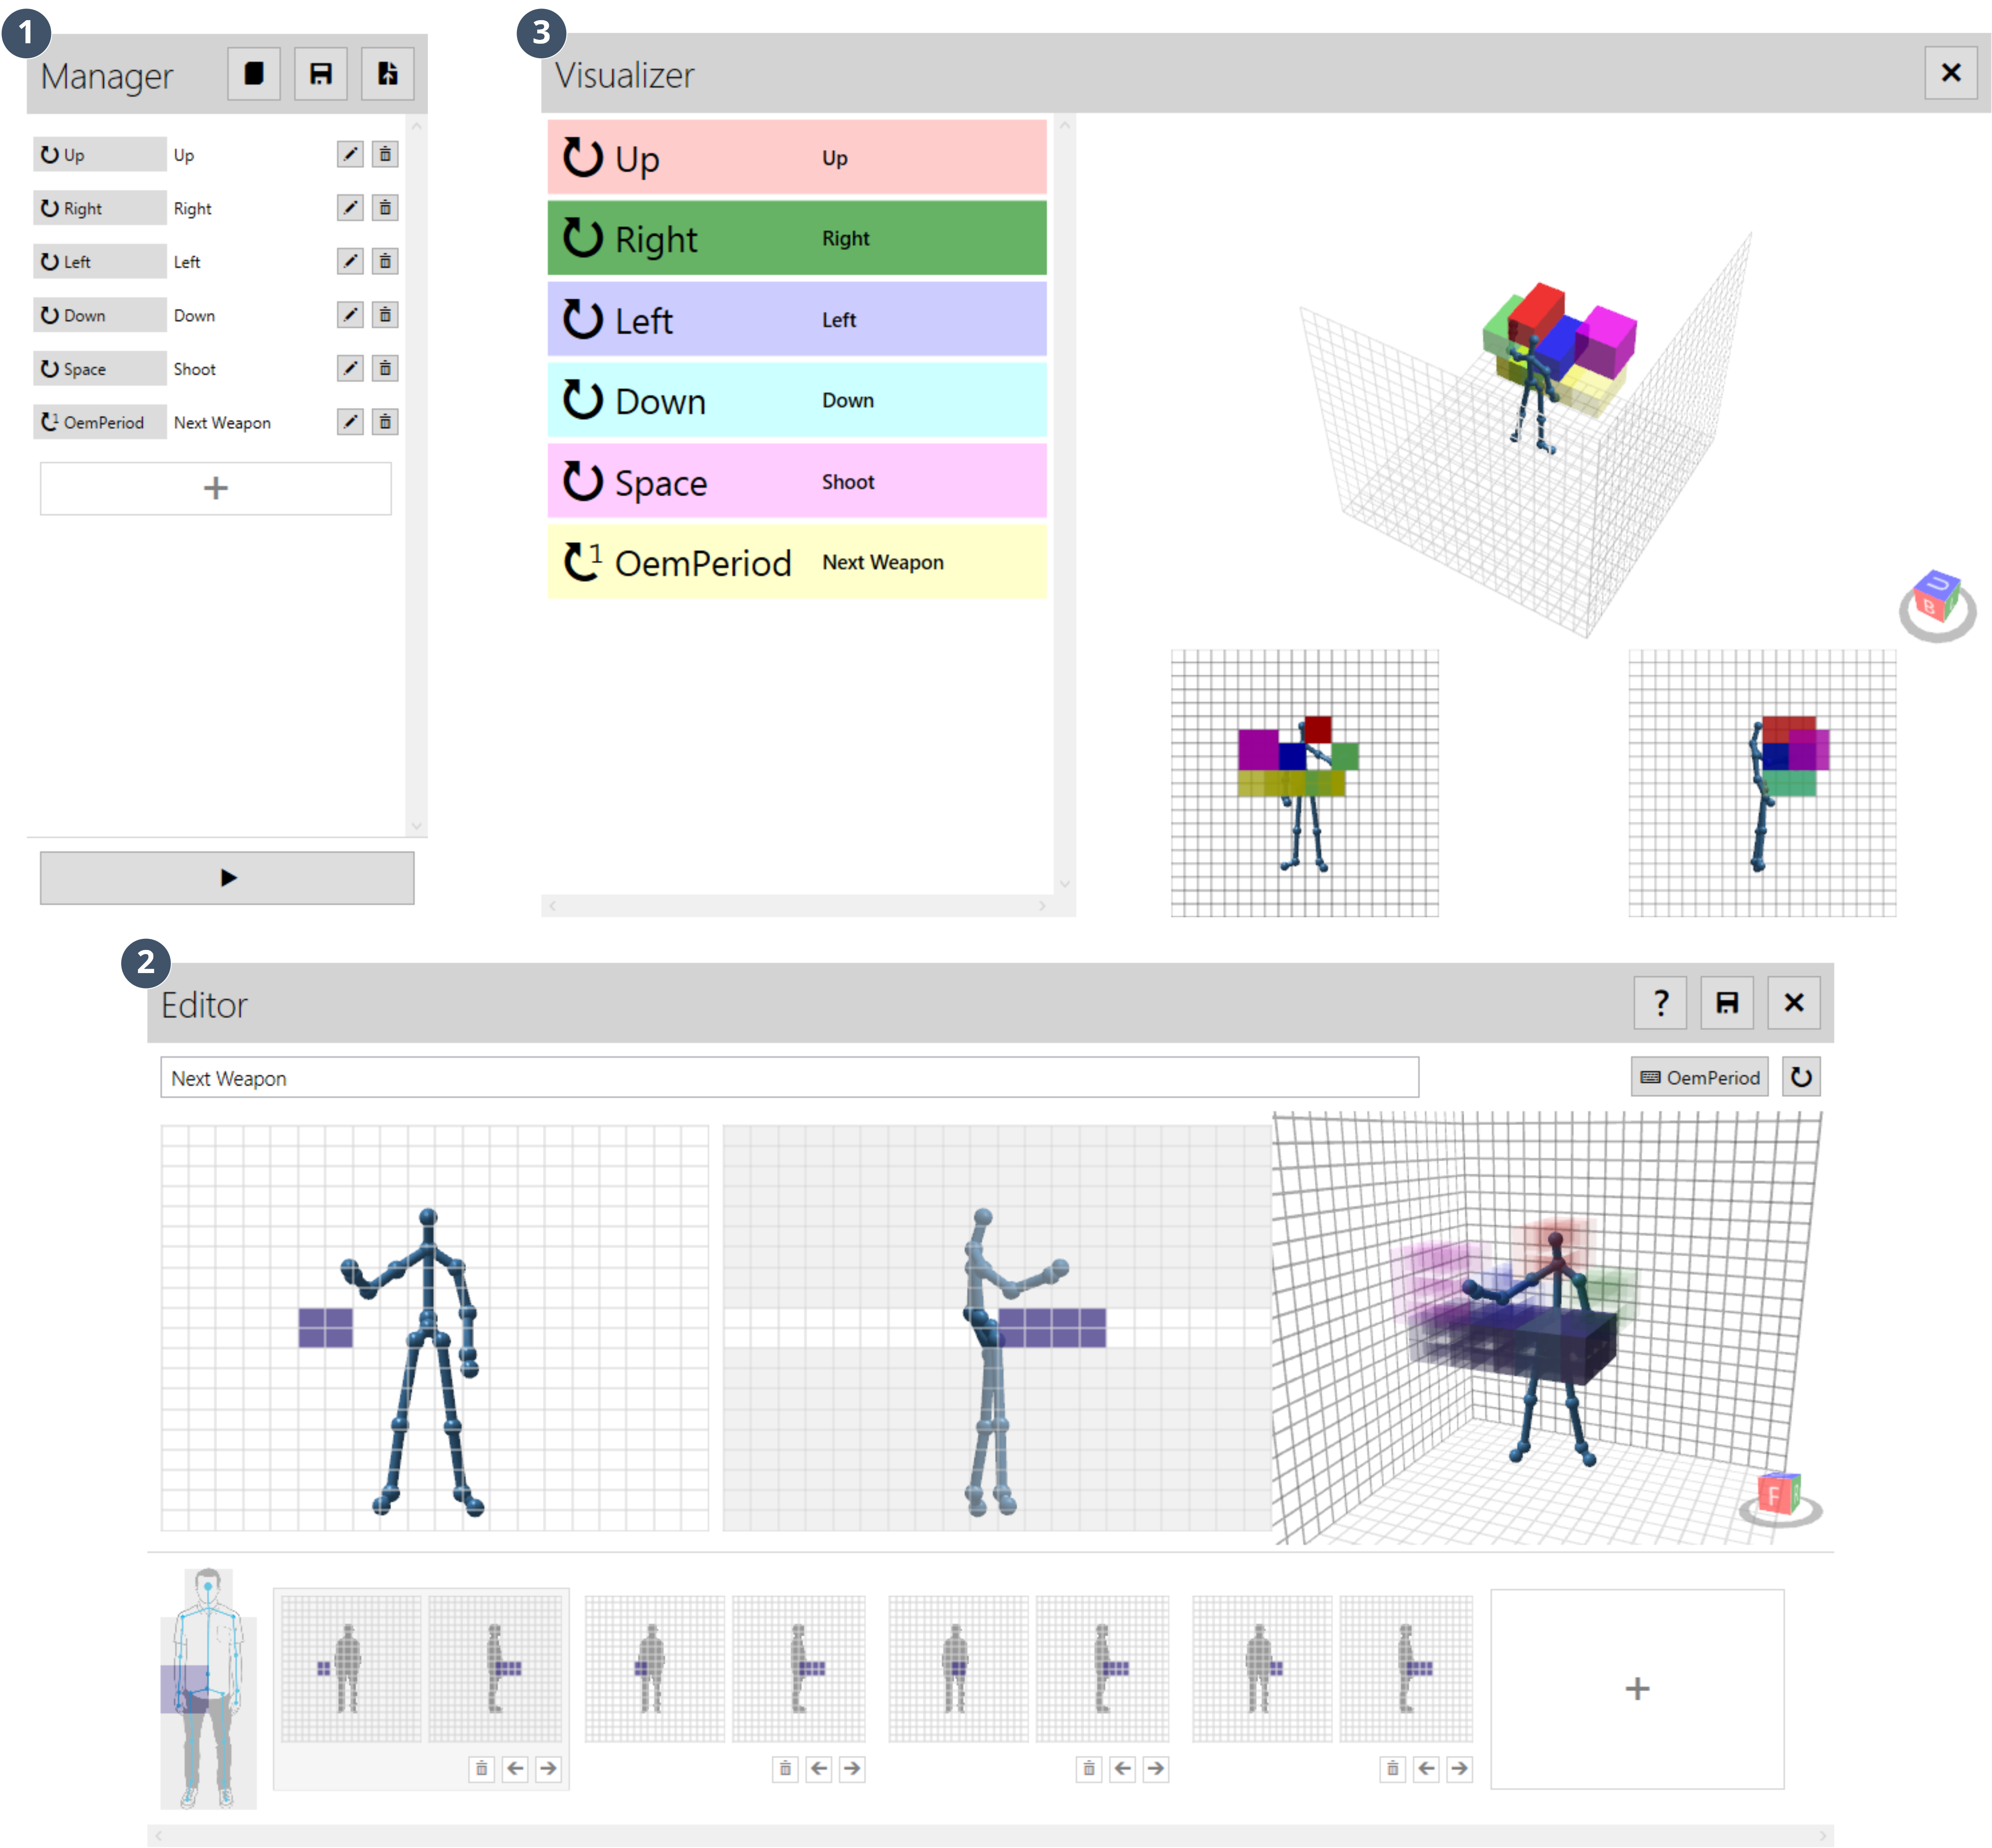
\includegraphics[width=\textwidth]{hotspotizer-modules}
\caption{Hotspotizer consists of three modules: (1) The Manager lists all of the gestures in the current collection and allows creating, saving and loading collections as well as adding, removing and editing individual gestures. (2) The Editor is the main workspace where gestures are authored. (3) The Visualizer provides interactive feedback on available and recognized gestures.}
\label{fig:hotspotizer-modules}
\end{figure}

\subsubsection{Creating and Editing Gestures}

Hotspotizer greets Ali with the Manager module containing empty gesture collection upon launch. Ali creates a new gesture in the collection, launching the Editor module \textbf{(1)}. Here, Ali assigns a name for the gesture for easy recall, specifies the Page Down key to be triggered when the gesture is performed, and confirms that the \emph{loop} toggle button is not checked – otherwise performing the gesture and holding the tracked limb over the hotspots in the last frame continues to hold down the keyboard key assigned to the gesture \textbf{(2)}.

Ali moves on to the main workspace where they use the front- and side-views over a representation of the tracked user to mark the positions of the hotspots for the first frame. Initially, all of the cells in the side view are disabled and grayed out. Marking cells on the front view enables the corresponding rows on the side view, whereupon Ali can mark the vertical and depth-wise position of their hotspots. Once hotspots are specified in all three dimensions by using these two grids, they appear on the 3D viewport on the right.

Once Ali completes marking the first frame’s hotspots, they can proceed to add another frame using the button next to the timeline of keyframes, and then another \textbf{(3)}. Finally, after marking the second and third frames’ hotspots, Ali selects the left hand as the limb that will be used in performing this gesture.

After saving the first gesture into the collection, Ali is taken back to the Manager module where they can add the remaining gestures and see the existing gestures to review, edit or delete them \textbf{(5)}. Once they are satisfied with the gesture collection they created, Ali can save the collection into a file for later use \textbf{(6)}.

\begin{sidewaysfigure}
\centering
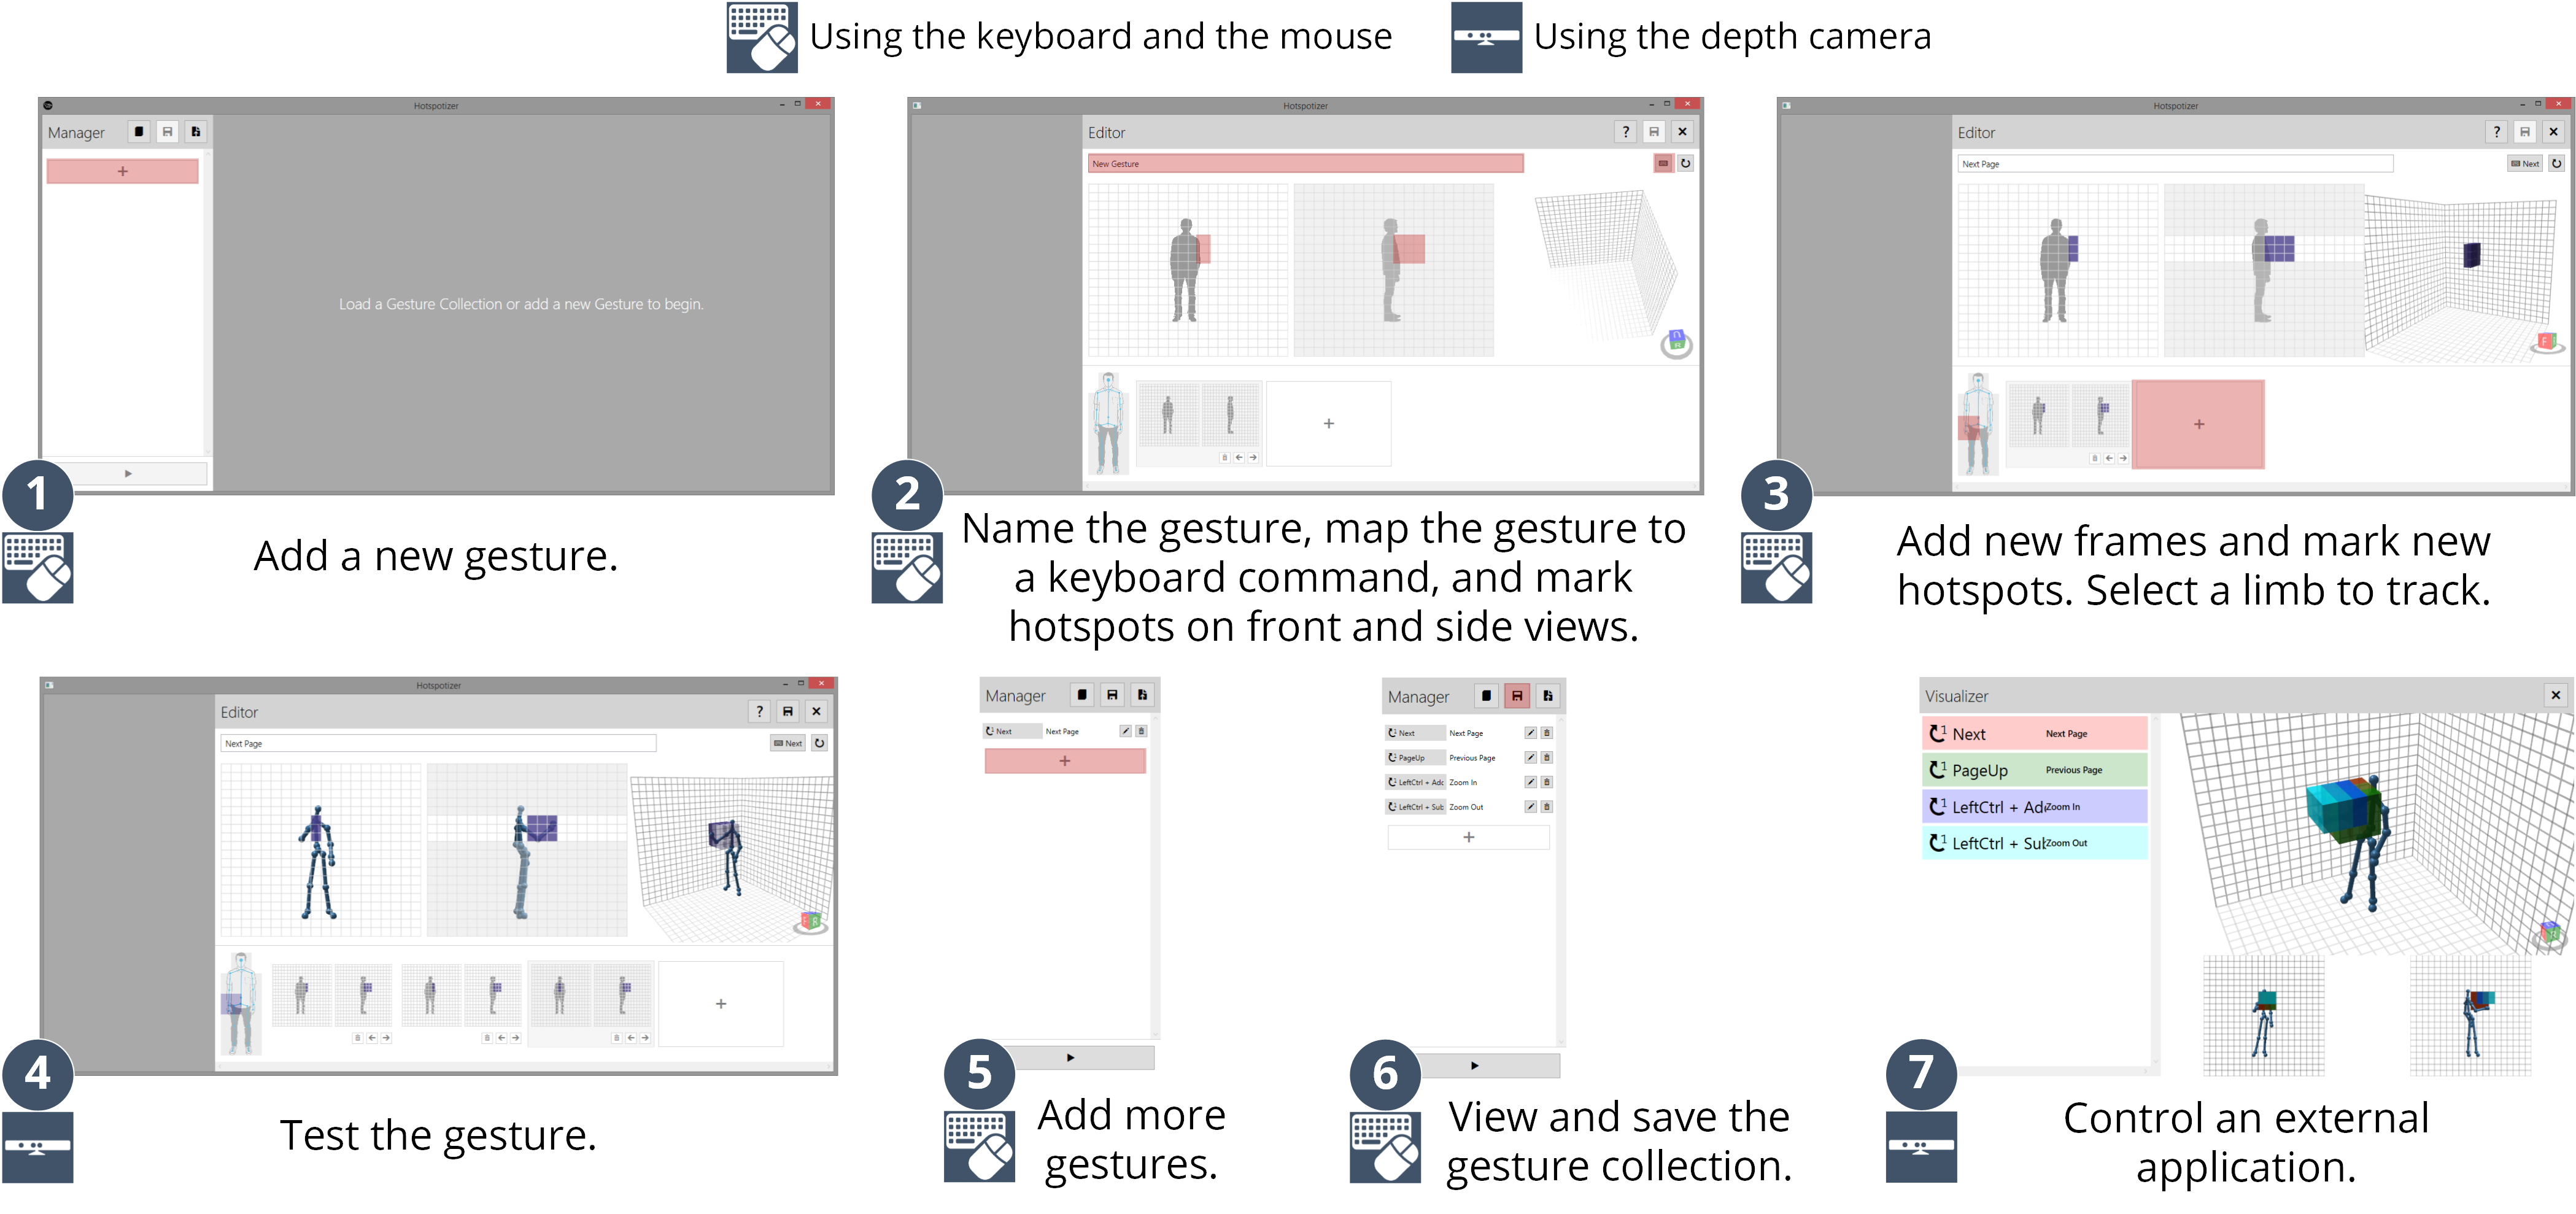
\includegraphics[width=.9\textwidth]{workflow}
\caption{The workflow of an end-user authoring gestures in Hotspotizer.}
\label{fig:workflow}
\end{sidewaysfigure}

\subsubsection{Testing Designs and Controlling External Applications}

At any time when using the Editor module, if they have a Kinect sensor connected to the computer, Ali may step in front of the sensor and see a rendering of the skeletal model of their body on the front, side and 3D viewports \textbf{(4)}. This feature can be used to rapidly test and tune hotspot locations at design time.

Testing over the whole gesture collection is available through the Visualizer module \textbf{(7)}. This module depicts a list of the gestures in the current collection and all of their hotspots on 3D, front and side viewports. Each gesture is shown in a different color. On the 3D viewport, transparency implies the order of hotspots. Hotspots glow when the tracked limb enters them in the correct order.

The Visualizer module also embeds the keyboard simulator. Launching the visualizer attaches a virtual keyboard to the system, which relays associated key events upon the successful performance of gestures. The visualization and the emulator continue to work when Hotspotizer is not in focus or is minimized.

\begin{SCfigure}[\sidecaptionrelwidth][t]
\centering
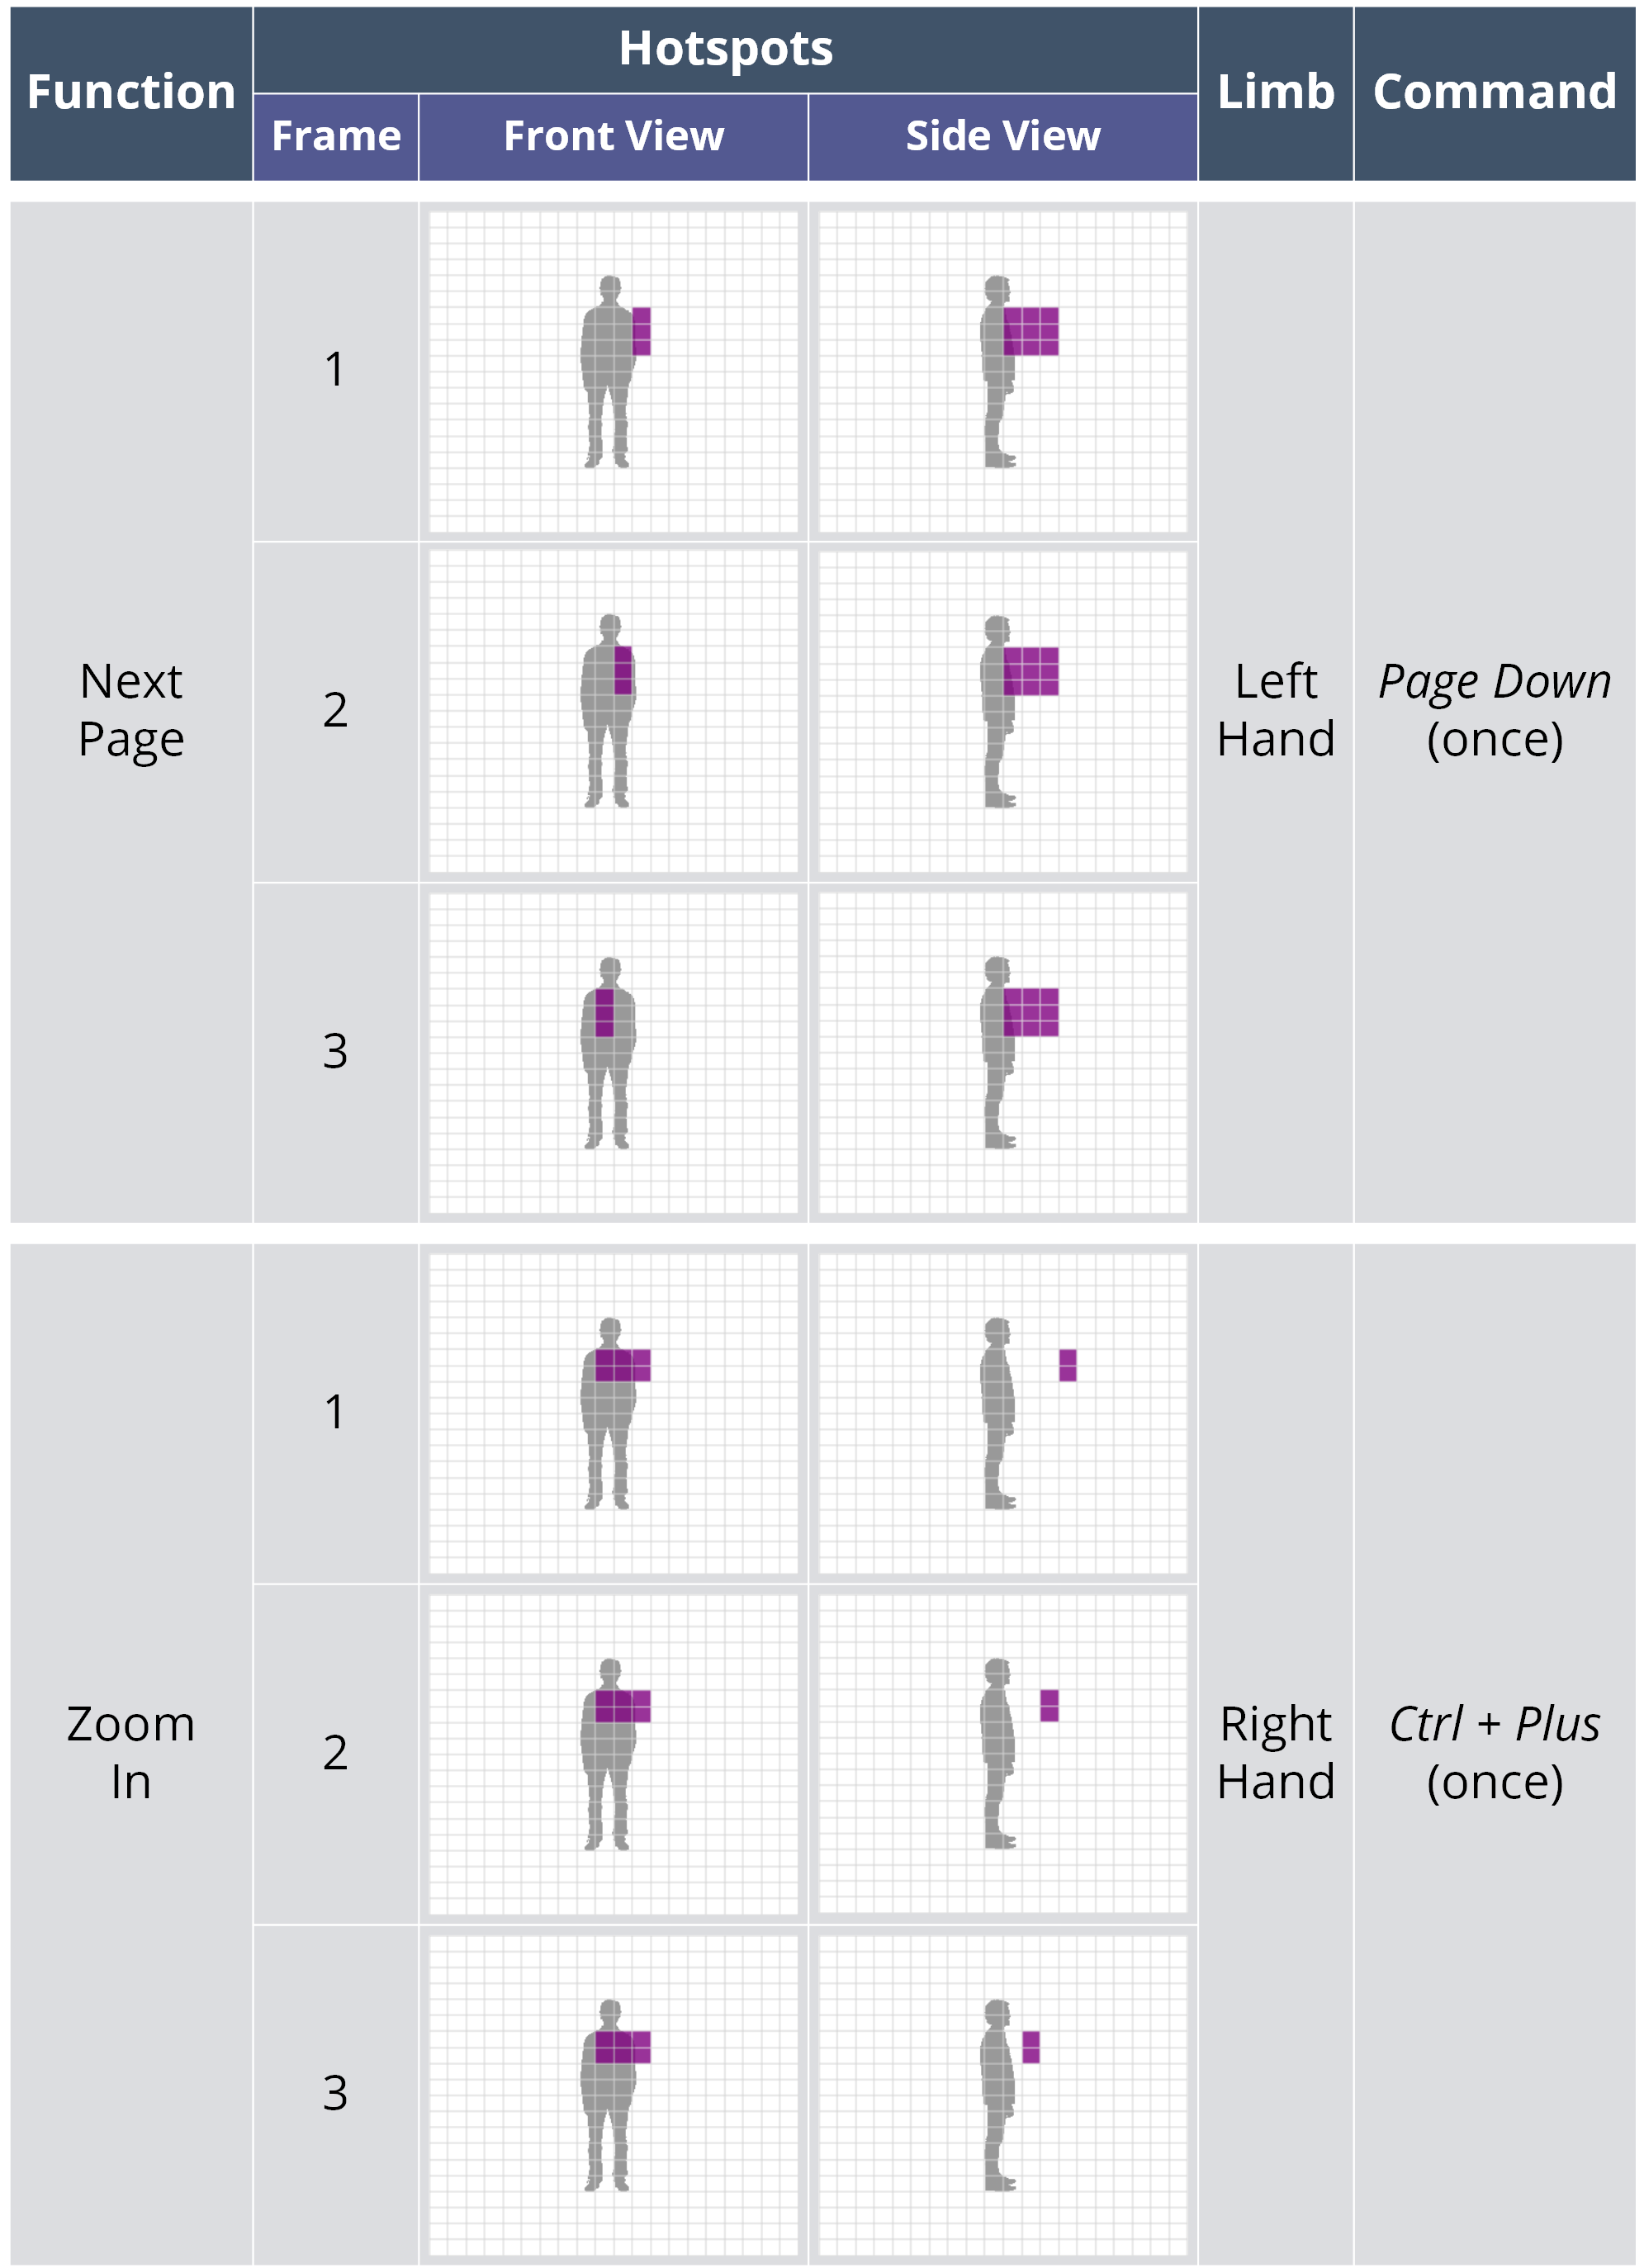
\includegraphics[width=.6\textwidth]{gestures}
\caption{\emph{Next page} and \emph{zoom in} gestures to control a document viewing application and the keyboard functionality that they map to. The diagrams show, respectively, hotspot arrangements for a swipe gesture and a beckoning motion.}
\label{fig:gestures}
\end{SCfigure}

\subsection{Space Discretization Specifics}

In the current implementation, the space around the skeletal model tracked by the Kinect sensor is partitioned into cubes that are 15cm on each side. The total workspace is a large cube that is 3m on each side. While this is much larger than both the horizontal and vertical reach of many people; this is by design, to accommodates unusually tall users. The centroid of the cube that comprises the workspace is affixed to the "hip center" joint returned by the Kinect sensor, which roughly corresponds to the centroid of the user's body. By specifying and tracking joint movements relative to the user’s skeletal model rather than the sensor’s position in real space, the user interfaces leverages the user’s sense of proprioception \parencite{Shoemaker:2010} in gesturing.

To describe gestures, the cubic cells within the workspace are marked to become hotspots – or \emph{hotspotized} – that register when a specified limb passes through them. Hotspotizing is accomplished by using front and side views in the Editor workspace. The front view is used to specify the horizontal and vertical positions of the hotspots. The side view is used to confirm the vertical and specify depth-wise positions. The design of this interaction style was inspired by architectural and engineering drawings.

Limbs available for tracking are the hands, feet, elbows, knees and the head. Each gesture can track only one limb. The design of user interface for authoring gestures that utilize multiple limbs without embodying excessive complexity can be explored in future work (see Section~\ref{sec:future-work}).

In order to enable the authoring of dynamic movements along with static poses, movements are split into discrete keyframes. A timeline in the Editor module shows the keyframes and allows adding, removing, reordering and editing actions. Hotspots within subsequent frames do not need to be adjacent, but the frames need to be traversed in the correct order and within a certain time limit for a gesture to be recognized. The inter-frame timeout in Hotspotizer is pre-set to 500ms. If more than 500ms elapses between a tracked limb engaging hotspots of subsequent frames, the gesture is not recognized. In order to relieve the user interface from complexity, this parameter has not been made adjustable.

The space discretization technique supports a versatile array of features. The size of hotspots could be made adjustable, even adaptive; to allow for fine gesturing close to the user’s body and more relaxed gesture boundaries at a distance. The total workspace volume could be made adjustable. The workspace could be defined in reference to limbs other than the center or in reference to the environment; supporting whole-body movements, a larger interaction space and rich proprioceptive interactions. Temporal constraints could be made adjustable or adaptive to allow designs that exploit velocity and acceleration in gesturing. Hotspotizer does not implement these features. The design of the interface focuses on rapid development, simplification of expertise and lowering of skill barriers. Through pre-adjusted parameters for space discretization and timing, the complexity of the gesture authoring process has been reduced and  the capabilities of the sensor are encapsulated within the interface. Future work may investigate empowering expert users with adjustability while maintaining the value added for non-experts.

\clearpage

\subsection{Implementation Details}

Hotspotizer was written in the \emph{C\#} programming language\footnote{\href{http://msdn.microsoft.com/en-us/library/kx37x362.aspx}{msdn.microsoft.com/library/kx37x362}}, using the \emph{Microsoft .NET Framework 4.5}\footnote{\href{http://www.microsoft.com/net}{microsoft.com/net}} and the \emph{Windows Presentation Foundation (WPF)}\footnote{\href{http://msdn.microsoft.com/en-us/library/ms754130.aspx}{msdn.microsoft.com/library/ms754130}} subsystem therein to create the user interface.

The following open source packages were used:

\begin{itemize}
\item \emph{Windows Input Simulator}\footnote{\href{http://inputsimulator.codeplex.com/}{inputsimulator.codeplex.com}} for keyboard emulation;
\item \emph{Json.NET}\footnote{\href{http://json.codeplex.com/}{json.codeplex.com}} for reading and writing gesture data to files; and,
\item \emph{Helix 3D Toolkit}\footnote{\href{http://helixtoolkit.codeplex.com/}{helixtoolkit.codeplex.com}} for 3D graphics.
\end{itemize}

Hotspotizer runs on Microsoft's \emph{Windows 7} and \emph{Windows 8} operating systems and requires the \emph{Microsoft Kinect Runtime}\footnote{\href{http://www.microsoft.com/en-us/download/details.aspx?id=40277}{microsoft.com/download/details.aspx?id=40277}}, and, if used with an \emph{Xbox Kinect} sensor, the \emph{Kinect SDK}\footnote{\href{http://www.microsoft.com/en-us/download/details.aspx?id=40278}{microsoft.com/download/details.aspx?id=40278}} to be installed on the user's computer.

Care has been taken to make the process of installing and running Hotspotizer as straightforward as possible, in order to accommodate diverse user populations. Hotspotizer is packaged as a Windows application that can, as convention dictates, be installed from a single executable installer file, launched from the \emph{Start Menu}, and uninstalled from the operating system's \emph{Control Panel}. Upon launch, Hotspotizer checks for its external requirements, the Kinect Runtime and SDK. If the requirements are unavailable, it prompts the user to install them, providing links to the web pages where they can be downloaded (Figure~\ref{fig:warning-message}).

\begin{SCfigure}[3][t]
\centering
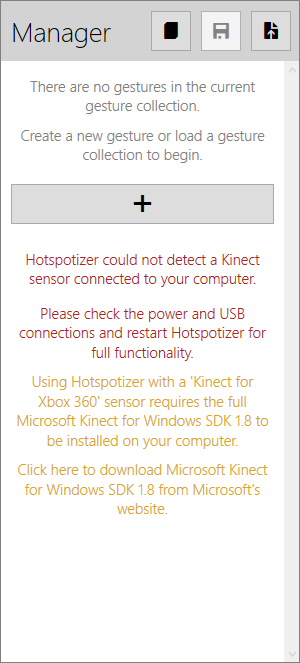
\includegraphics[width=.25\textwidth]{warning-message}
\caption{If the Kinect sensor is not functioning properly or if pre-requisite software is not installed on the computer, Hotspotizer prompts the user with a warning message.}
\label{fig:warning-message}
\end{SCfigure}

\subsection{Discussion}

The space discretization paradigm and its current implementation in Hotspotizer feature strengths and limitations that manifest as side effects of design choices.

One strength of the implementation is that gesture recognition is not influenced by the user's position and orientation within the sensor's field of view, provided that the depth image is not distorted and the sensor can build an accurate skeletal model of the user. Since the discretized workspace is affixed to the user's hip, hotspot locations are defined relative to the user's own body and the traversal of hotspots is detected properly as long as the skeletal model is built correctly. As a limitation of the depth sensor, skeletal modeling fails under certain conditions; e.g. the user turning their back to the sensor or engaging in contortions, the presence of objects that resemble a human form in the sensor's field of view, etc. Hotspotizer automatically hides the skeletal representation and halts gesture recognition when failures occur, and resumes operation when the sensor provides a skeletal model.

Certain limitations result from the design choice to prioritize leveraging a common infrastructure for end-users by mapping gestures to keyboard events. This obscures what \textcite{Hartmann:2007} call "association semantics" --- i.e. the relationship between commands relayed to applications from Hotspotizer and the resulting application behaviors --- and limits the expressive power of the gesture authoring paradigm.

A further limitation is that Hotspotizer currently does not support authoring continuous --- or \emph{online} \parencite{Hoste:2014} --- gestures that affect some variable while they are being performed (as opposed to \emph{offline} gestures that execute commands when the gesture is performed from the beginning to the end). This is not a limitation of the space discretization paradigm; since, theoretically, smaller portions of a gesture could be assigned to affect continuous variables (albeit in a quantized manner). Likewise, gestures that involve pointing at or manipulating dynamic user interface components in third party applications are not supported. This could be overcome by linking the discretized space model around the user with the virtual space of the user interface. However, these features require integration with a fully featured programming environment or language, which is beyond the design goals for this project. Exploring "tighter integration with application logic" \parencite{Hartmann:2007} to empower software developers is a goal for future work.
